\chapter{Evaluation}
\label{chap:Evaluation}

To measure the effectiveness of dynamic windowing for multi-stream operators during the 
mapping of non-RDF heterogeneous data we need to measure the following 
metrics of our stream processing framework: \emph{latency}, \emph{throughput},
\emph{memory usage}, and \emph{completeness}. In this paper \emph{Throughput} refers to the number of processed input records per second.
\emph{Latency, throughput,} and \emph{memory usage} are measured following the recent benchmark studies by 
Van Dongen and Van den Poel(2020)~\cite{evalution_of_spe}. 
However, to evaluate 
for the \emph{completeness}
of the generated output, a reference output needs 
to be generated for comparison. Since a data stream is unbounded and cannot be processed completely to check for \emph{completeness}, we use a bounded 
dataset of relatively large volume to measure \emph{completeness}.
To ensure consistency in the complexity of the multi-stream operator being used, 
we apply the join operator in the windows --- a common operator used in 
data enrichment scenarios. All attributes that are common in both 
input are used as \emph{key} attributes for joining, 
to reduce the output size and keep the completeness measurement as concise 
as possible. Using less \emph{key} attributes would just lead to a significant increase 
in the number of redundant duplicate triples generated for completeness measure. 

The following sections describe the workloads and the data used to evaluate the
different metrics. Setups required to reproduce the evaluation are elaborated on
in their respective sections. 


\section{Data}

Assessment of our dynamic windowing scheme for multi-stream operator requires 
the data streams to have some common attributes to enrich the data. Furthermore, to 
mirror a real-world scenario, we employ data gathered from IoT sensors. 
We use the same data 
as the benchmark in the paper by Van Dongen and Van den Poel~\cite{evalution_of_spe}. 
The data is provided by NDW (Nationale Databank Wegverkeersgegevens) from the 
Netherlands~\footnote{NDW data site: \href{http://opendata.ndw.nu/}{http://opendata.ndw.nu/} }.
It consists of measurements of the number of cars and their average speed across the different 
lanes on a highway. 
The sensor data was replayed by a Kafka publisher into two topics 
\emph{ndwflow} and \emph{ndwspeed}, for the number of cars and the average speed respectively. The json 
structure for the records from each stream are shown in Listing~\ref{lst:record_json_structure}. 

\begin{lstlisting}[language=JSON, 
caption={JSON data structure of the records.}, 
label={lst:record_json_structure} ]

//NDWSpeed topic's record structure
{
    "internalId": "lane1", 
    "lat":51.41268,
    "long":5.42929,
    "speed":92,
    "accuracy":100,
    "timestamp":"2021-04-01 17:58:10",
    "num_lanes":1
}

// NDWFlow topic's record structure
{
    "internalId": "lane1", 
    "lat":51.41268,
    "long":5.42929,
    "flow":360,
    "period":60,
    "accuracy":100,
    "timestamp":"2021-04-01 17:52:22",
    "num_lanes":1
}
\end{lstlisting}




\section{Evaluation setup}

Docker\footnote{Docker: \url{https://www.docker.com}} is used to package 
our applications in separate containers. The docker setup with the containers 
is illustrated in Figure~\ref{fig:docker_setup}. The docker containers 
are run on a standalone machine in order to mitigate the influence of 
network communication as much as possible. Apache Kafka is used 
as the message broker for our data. The setup for the Kafka broker is 
the same as described in \cite{evalution_of_spe}. Message replication 
is disabled to prevent heavy load on the Kafka broker. 

In order to measure the metrics without significant influence from  
Apache Flink's configuration, we kept the default values as much as possible. 
Table~\ref{tab:computer_specs} describes the configuration for the 
Apache Flink to run our RMLStreamer with window implementations. We 
disabled checkpointing since we are only evaluating the performance of 
the window on processing the stream, not fault tolerance. Enabling 
fault tolerance would have negative impact on latency measure 
with the extra overhead from checkpointing. Thus, the 
default InMemoryStateBackend is enough for this evaluation without 
fault tolerance.

Watermarks are emitted every 50ms and object reuse is enabled to 
mitigate the performance impact incurred by redundant object creations just 
like in ~\cite{evalution_of_spe}. 

\subsection{Metrics measurement}%
\label{sub:Metrics measurement}

CPU usage, throughput, memory, and latency exposed 
by Flink's Rest API, are constantly polled every 100ms by a 
Python script scraper.
CPU usage, throughput 
and memory usage are measured internally by Flink,
while latency measurement 
is implemented manually using Flink's Metrics API to more accurately measure the amount of 
time spent in the window by a record before being processed. The accuracy of the 
measurements depends on the default internal metric update interval by Flink.
The aforementioned metrics are averaged across the parallelized window operators since 
Flink spreads the operations across the available task slots of Taskmanager. 
Intersection over union (IOU) is used as the metric to measure the completeness
of the joined result generated by the windows.  

For \emph{CPU usage}, \emph{throughput}, and \emph{memory}, we drop the first 10 min of 
measurements because of the overhead of the warm up period of the JVM for RMLStreamer. 
The 10 min of measurement is derived after analyzing measurements from 
different runs. The average amount of time taken 
for the start of a stable pattern in the metric measurements is taken as 
the 10 min threshold limit. 
However, it might still be interesting to observe the stabilization of latency pattern by the 
different windows implementation. Therefore, latency measurement is done throughout the 
lifetime of the evaluation workload. 

\subsubsection{CPU usage}%
\label{ssub:CPU usage}
For CPU usage, we measure Taskmanager's CPU usage, since it is 
the one responsible for executing the RMLStreamer code. The CPU usage is 
monitored at the Taskmanager level. 

\subsubsection{Throughput}%
\label{ssub:Throughput}
Throughput measurement is defined as the number of records processed by the 
window operator per second. 
It is measured at the output of the window operator, since we want to measure 
output performance of the window operators. 


\subsubsection{Memory usage}%
\label{ssub:Memory usage}
Due to limitation in granularity of measurement in Flink, 
JVM heap memory used by the job is used to estimate the memory usage of window 
operator. We expect the memory usage by other operators in the job to be 
consistent and low across the different evaluation since they are stateless operators.
Therefore, measurement of JVM heap memory is a good enough estimate for memory usage 
of window operators for storing the state. 


\subsubsection{Latency measurement}%
\label{ssub:Latency measurement}
We measure the latency by attaching a processing timestamp to the records before they enter the window. 
Once the records are processed and emitted after the join, the difference 
between the current processing time and the attached old processing time 
is taken as the \emph{latency} for the records. This enables accurate measurement of
the amount of time spent in the window since the measurement is done on the 
same machine with the same clock. However, there is a subtle difference
in the \emph{latency} calculation between the Tumbling and Dynamic window.


This is due to the difference in the \emph{trigger} policy between the two windows. 
Dynamic window fires the \emph{trigger} event immediately, once it receives a record, 
to process it and emit the joined results as a batch. This means that we need to measure the 
\textbf{minimum} latency amongst the records being emitted in the joined records batch. 
Tumbling window fires the \emph{trigger} event only when it has to \emph{evict} the window. 
Therefore, there is no joined results generated before the eviction of the records 
inside the window; we have to measure the \textbf{average} latency of the records in the joined 
records batch. 

\subsubsection{Completeness measurement}%
\label{ssub:Completeness measurement}
Evaluating completeness requires a dataset which could be mapped completely by a static 
mapping engine. For our evaluation, this dataset will be the same set of data used to 
evaluate the window implementation in a streaming environment. These streamed data are 
stored in the Kafka topics as long as the Kafka broker is alive. 
To generate \emph{bounded} input data for 
the static mapping engine, we could write the stored data from the topics 
into a file on disk. This input data is processed by RMLStreamer in bounded data 
processing mode to generate the \emph{complete} set of triples. 
This set of output triples will be generated according 
to the RML mappings defined for bounded data (Appendix~\ref{lst:bounded_mapping_file}). 

Streaming data is also usually 
ordered according to the event time (Chapter~\ref{chap:data_stream_processing}) 
and the same entity could appear in the 
stream at a different timestamp. This can lead to duplicates in the generated output by 
the bounded data processing. We need to preserve these duplicates in the 
output since they are valid records produced by the data sources and duplicates are 
expected in streaming data. The duplicate preservation for the generated 
output triples by the bounded data processing
is achieved by disabling 
the duplicate filtering from the bounded data processing. 


The generated output triples from the evaluation of the windows, and the bounded data processing are 
used to calculate the IOU metric to measure the similarity between the two outputs.    


\section{Window Configurations}
\label{sec:Window Configurations}
The windows are configured according to Table~\ref{tab:window_configuration}. 
Dynamic window is configured with the same initial window size as the 
Tumbling window to ensure that Dynamic window is not processing too little or too much 
records in the first few minutes. 


\begin{figure}[htpb]
    \centering
    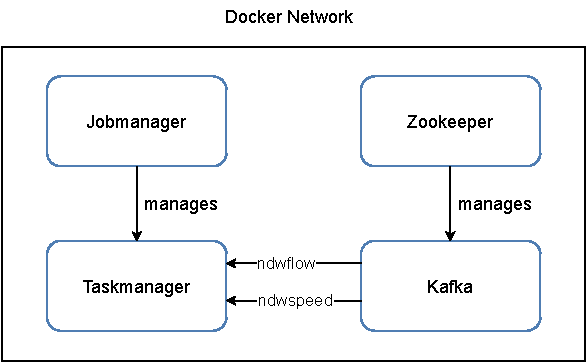
\includegraphics[width=0.8\linewidth]{fig/docker_setup.pdf}
    \caption[Setup of application containers inside the same docker network.]{ 
Setup of application containers inside the same docker network.
The kafka topics \emph{ndwflow} and \emph{ndwspeed} are consumed by the 
RMLStreamer job inside the Taskmanager.}
    \label{fig:docker_setup}
\end{figure}

\begin{table}[htbp]
    \centering
    \begin{tabular}{|c|c|c|}
        \hline
        \textbf{Parameter}        & \textbf{Default} & \textbf{Value}  \\ \hline
        JobManager count          & /                & 1               \\ \hline
        TaskManager count         & /                & 1               \\ \hline
        JobManager CPU cores      & /                & 2               \\ \hline
        TaskManager CPU cores     & /                & 5               \\ \hline
        TaskManager heap / memory & 512 MB / 1.7 GB  & 512 MB / 1.7 GB \\ \hline
        Number of task slots      & 1                & 4               \\ \hline
        Default parallelism       & 1                & 4               \\ \hline
        StateBackend              & InMemory         & InMemory        \\ \hline
        Checkpoint Interval       & None             & None            \\ \hline
        Time characteristics      & processing time  & event time      \\ \hline
        Watermark interval        & /                & 50ms            \\ \hline
        Object reuse              & disabled         & enabled         \\ \hline
    \end{tabular}
    \caption{Apache Flink's configuration.}
\label{tab:computer_specs}
\end{table}

\begin{table}[htbp]
    \centering
    \begin{subtable}{\textwidth}
        \centering
        \begin{tabular}{|r|c|}
        \hline
        Parameter   & Value           \\ \hline
        Window size & 2s (Event time) \\ \hline
        \end{tabular}
        \caption{Tumbling Window's configuration }
        \label{tab:tumbling_config}
    \end{subtable}


    \begin{subtable}{\textwidth}
        \centering
        \begin{tabular}{|r|c|}
        \hline
        \multicolumn{1}{|c|}{Parameter}               & Value             \\ \hline
        $\epsilon_l$            & 1.2               \\ \hline
        $\epsilon_u$            & 0.8               \\ \hline
        Initial window size     & 2s (Event time)   \\ \hline
        Upper window size limit & 5s (Event time)   \\ \hline
        Lower window size limit & 50ms (Event time) \\ \hline
        \end{tabular}
        \caption{Dynamic Window's configuration}
        \label{tab:dynamic_config}
    \end{subtable}

    \caption{Configuration of the windows used for evaluation.}
    \label{tab:window_configuration}

\end{table}
\newpage

\section{Evaluation pipeline}
\begin{figure}[!htbp]
    \centering
    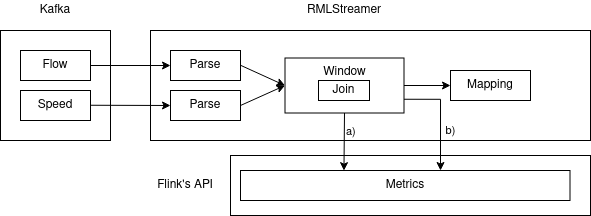
\includegraphics[width=\textwidth]{fig/evaluation_architecture.png}
    \caption{Evaluation flow based on~\cite{evalution_of_spe} with some changes to only 
    take metrics at the "Join" stage.
    a) \emph{latency, memory}, and \emph{cpu usage} of evaluating the join operator in windows.
    b) \emph{throughput} of the generated output triple.}
    \label{fig:evaluation_flow}
    
\end{figure}

Similar to the workflow process in~\cite{evalution_of_spe, benchmark_sce}, we set up
our evaluation pipeline as illustrated in Figure~\ref{fig:evaluation_flow}. Setting it 
up according to the illustrated pipeline allows us to have fine control over the 
workload scenarios and to narrow the scope of the metrics to the windows only. 




\section{Workload scenarios}
\label{sec:workload}
Data streams have characteristics 
which determine the performance of stream processing frameworks and its 
operators (Chapter~\ref{chap:data_stream_processing}). Therefore, 
there is a need to evaluate our dynamic window implementation under different workload scenarios. 
These workloads are similar to the ones used in~\cite{evalution_of_spe} where relevant.

\subsection{Workload for latency measurement}
As described in the paper by Van Dongen and Van den Poel~\cite{evalution_of_spe}, 
\emph{throughput} and \emph{latency} can affect each other if the workload is 
improperly configured. Therefore, measurement of the \emph{latency} caused only 
by the window implementations, requires the stream processing framework not to be 
stressed by significant \emph{throughput}. Thus, the Kafka broker 
publishes the records at a very low constant rate of around 400 messages per second for 
this workload. 


\subsection{Workload with periodic burst}
Fluctuation in the streaming sources are normal with unstable network connections. 
The windowing operator must therefore cope with sudden changes in the 
fluctuation of the velocity of the data stream. This workload attempts to emulate 
the scenario where multiple IoT devices send data in bursts with a periodic 
time interval. The workload has a constant low stream rate with an occasional 
burst of data. Therefore, 38 000 records will be published every 10 seconds which 
takes around 170ms to 180ms since the time taken to publish can deviate based on the 
load of the Kafka brokers. 


\subsection{Workload for completeness}
The implementation of the dynamic window should also ensure that the generated 
output is as \emph{complete} as possible. 
Depending on the type of window being used, \emph{completeness} of the output will be
affected by the window size. If the window size is not sufficiently large to handle 
the input velocity, the next incoming record will be processed in the new window instead of 
the old window where it is more relevant. Thus, 
we will use two stream rates, constant and periodic, to measure the \emph{completeness} of the results generated 
by the different windows. The stream rates for constant and periodic are the same as their 
workloads previously mentioned; 400 messages per second for \emph{constant rate} and 
\emph{periodic burst} of 38 000 messages at every 10th second with 400 messages per second 
between each burst.

As described in Section~\ref{ssub:Completeness measurement}, 
the input data for this workload will be derived from the respective workloads with 
constant and periodic stream rate. We will write out the input data to a file, from the relevant Kafka 
topics \emph{ndwflow} and \emph{ndwspeed}, after each evaluation run of the two windows implementation. 





